% =============================================================================
% Exit Survey Results — Economics & Finance Workshop
% Consultant-style summary of student exit-survey feedback (n = 12)
% Compile: cd output/surveys && TEXINPUTS=../../codes/Preambles:$TEXINPUTS xelatex exit_survey_results.tex
% =============================================================================
\documentclass[letterpaper,10pt]{article}
% =============================================================================
% Pathways: Economics & Finance Workshop — Document Preamble
% =============================================================================
% Usage: Each handout/activity .tex file should start with:
%   \documentclass[letterpaper,10pt]{article}
%   % =============================================================================
% Pathways: Economics & Finance Workshop — Document Preamble
% =============================================================================
% Usage: Each handout/activity .tex file should start with:
%   \documentclass[letterpaper,10pt]{article}
%   % =============================================================================
% Pathways: Economics & Finance Workshop — Document Preamble
% =============================================================================
% Usage: Each handout/activity .tex file should start with:
%   \documentclass[letterpaper,10pt]{article}
%   \input{../../codes/Preambles/header_doc}
% Compile: cd output/Handouts && TEXINPUTS=../../codes/Preambles:$TEXINPUTS xelatex file.tex
% =============================================================================

% ---------- Packages ----------
% Fonts
\usepackage{palatino}
\usepackage[utf8]{inputenc}
\usepackage[T1]{fontenc}
\usepackage[normalem]{ulem}

% Math
\usepackage{amsmath,amssymb,amsthm,eucal,bbold,bm}

% Figures and tables
\usepackage{graphicx}
\usepackage{xcolor}
\usepackage{array,tabularx,booktabs,subcaption}
\usepackage{pdflscape}
\usepackage{siunitx}

% TikZ and pgfplots
\usepackage{pgfplots}
\pgfplotsset{compat=1.18}
\usepackage{tikz}
\usetikzlibrary{positioning,arrows.meta,calc}

% Colored boxes
\usepackage[most]{tcolorbox}

% Miscellaneous
\usepackage{hyperref}
\usepackage{setspace}
\usepackage{enumitem}

% ---------- Margins ----------
\usepackage[left=1in,right=1in,top=0.75in,bottom=1in,marginparwidth=1.5in,footskip=0.7in]{geometry}

% ---------- Itemize ----------
\setlist[enumerate]{itemsep=-0.4em,topsep=0.2em}
\setlist[itemize]{itemsep=-0.4em,topsep=0.2em}

% =============================================================================
% Colors — Okabe-Ito colorblind-friendly palette
% =============================================================================

\definecolor{black}{HTML}{000000}
\definecolor{orange}{HTML}{E69F00}
\definecolor{skyblue}{HTML}{56B4E9}
\definecolor{green}{HTML}{009E73}
\definecolor{yellow}{HTML}{F0E442}
\definecolor{blue}{HTML}{0072B2}
\definecolor{vermillion}{HTML}{D55E00}
\definecolor{purple}{HTML}{CC79A7}

% Semantic aliases (mapped to Okabe-Ito)
\definecolor{softbg}{HTML}{F5F5F5}
\definecolor{lightgray}{gray}{0.65}

% =============================================================================
% Box Environments
% =============================================================================

% --- Key points (orange background) ---
\newtcolorbox{keybox}{
  colback=orange!12,
  colframe=orange,
  fonttitle=\bfseries,
  boxrule=0.5pt,
  arc=2pt,
  left=6pt,
  right=6pt,
  top=4pt,
  bottom=4pt
}

% --- Highlights (orange left accent) ---
\newtcolorbox{highlightbox}{
  colback=white,
  colframe=orange,
  fonttitle=\bfseries,
  boxrule=0pt,
  leftrule=3pt,
  arc=0pt,
  left=6pt,
  right=6pt,
  top=4pt,
  bottom=4pt
}

% --- Definitions (blue border, titled) ---
\newtcolorbox{definitionbox}[1][]{
  colback=blue!5,
  colframe=blue,
  fonttitle=\bfseries,
  title={#1},
  boxrule=0.5pt,
  arc=2pt,
  left=6pt,
  right=6pt,
  top=4pt,
  bottom=4pt
}

% --- Methods (sky blue background) ---
\newtcolorbox{methodbox}{
  colback=skyblue!8,
  colframe=skyblue!70,
  fonttitle=\bfseries,
  boxrule=0.5pt,
  arc=2pt,
  left=6pt,
  right=6pt,
  top=4pt,
  bottom=4pt
}

% --- Results (green border) ---
\newtcolorbox{resultbox}{
  colback=green!5,
  colframe=green,
  fonttitle=\bfseries,
  boxrule=0.5pt,
  arc=2pt,
  left=6pt,
  right=6pt,
  top=4pt,
  bottom=4pt
}

% --- Quotes (purple left rule) ---
\newtcolorbox{quotebox}{
  colback=softbg,
  colframe=purple,
  fonttitle=\itshape,
  boxrule=0pt,
  leftrule=2pt,
  arc=0pt,
  left=6pt,
  right=6pt,
  top=4pt,
  bottom=4pt
}

% =============================================================================
% Math Commands
% =============================================================================

\newcommand{\E}{\mathrm{E}}
\newcommand{\Var}{\mathrm{Var}}
\newcommand{\Cov}{\mathrm{Cov}}
\newcommand{\R}{\mathbb{R}}
\newcommand{\suminfty}[1]{\sum_{#1=0}^\infty}
\newcommand{\Lcal}{\mathcal{L}}
\newcommand{\prtl}[2]{\frac{\partial #1}{\partial #2}}
\renewcommand{\div}[2]{\frac{d #1}{d #2}}
\newcommand{\suchthat}{\text{ s.t. }}
\newcommand{\wrt}{\text{ w.r.t. }}
\newcommand{\red}[1]{\textcolor{vermillion}{#1}}
\newcommand{\blue}[1]{\textcolor{blue}{#1}}

% =============================================================================
% Economics Shortcuts
% =============================================================================

\newcommand{\OC}{\text{Opportunity Cost}}
\newcommand{\DWL}{\text{DWL}}
\newcommand{\pmark}{\textcolor{resultgreen}{\checkmark}}
\newcommand{\xmark}{\textcolor{darkred}{\texttimes}}

% Compile: cd output/Handouts && TEXINPUTS=../../codes/Preambles:$TEXINPUTS xelatex file.tex
% =============================================================================

% ---------- Packages ----------
% Fonts
\usepackage{palatino}
\usepackage[utf8]{inputenc}
\usepackage[T1]{fontenc}
\usepackage[normalem]{ulem}

% Math
\usepackage{amsmath,amssymb,amsthm,eucal,bbold,bm}

% Figures and tables
\usepackage{graphicx}
\usepackage{xcolor}
\usepackage{array,tabularx,booktabs,subcaption}
\usepackage{pdflscape}
\usepackage{siunitx}

% TikZ and pgfplots
\usepackage{pgfplots}
\pgfplotsset{compat=1.18}
\usepackage{tikz}
\usetikzlibrary{positioning,arrows.meta,calc}

% Colored boxes
\usepackage[most]{tcolorbox}

% Miscellaneous
\usepackage{hyperref}
\usepackage{setspace}
\usepackage{enumitem}

% ---------- Margins ----------
\usepackage[left=1in,right=1in,top=0.75in,bottom=1in,marginparwidth=1.5in,footskip=0.7in]{geometry}

% ---------- Itemize ----------
\setlist[enumerate]{itemsep=-0.4em,topsep=0.2em}
\setlist[itemize]{itemsep=-0.4em,topsep=0.2em}

% =============================================================================
% Colors — Okabe-Ito colorblind-friendly palette
% =============================================================================

\definecolor{black}{HTML}{000000}
\definecolor{orange}{HTML}{E69F00}
\definecolor{skyblue}{HTML}{56B4E9}
\definecolor{green}{HTML}{009E73}
\definecolor{yellow}{HTML}{F0E442}
\definecolor{blue}{HTML}{0072B2}
\definecolor{vermillion}{HTML}{D55E00}
\definecolor{purple}{HTML}{CC79A7}

% Semantic aliases (mapped to Okabe-Ito)
\definecolor{softbg}{HTML}{F5F5F5}
\definecolor{lightgray}{gray}{0.65}

% =============================================================================
% Box Environments
% =============================================================================

% --- Key points (orange background) ---
\newtcolorbox{keybox}{
  colback=orange!12,
  colframe=orange,
  fonttitle=\bfseries,
  boxrule=0.5pt,
  arc=2pt,
  left=6pt,
  right=6pt,
  top=4pt,
  bottom=4pt
}

% --- Highlights (orange left accent) ---
\newtcolorbox{highlightbox}{
  colback=white,
  colframe=orange,
  fonttitle=\bfseries,
  boxrule=0pt,
  leftrule=3pt,
  arc=0pt,
  left=6pt,
  right=6pt,
  top=4pt,
  bottom=4pt
}

% --- Definitions (blue border, titled) ---
\newtcolorbox{definitionbox}[1][]{
  colback=blue!5,
  colframe=blue,
  fonttitle=\bfseries,
  title={#1},
  boxrule=0.5pt,
  arc=2pt,
  left=6pt,
  right=6pt,
  top=4pt,
  bottom=4pt
}

% --- Methods (sky blue background) ---
\newtcolorbox{methodbox}{
  colback=skyblue!8,
  colframe=skyblue!70,
  fonttitle=\bfseries,
  boxrule=0.5pt,
  arc=2pt,
  left=6pt,
  right=6pt,
  top=4pt,
  bottom=4pt
}

% --- Results (green border) ---
\newtcolorbox{resultbox}{
  colback=green!5,
  colframe=green,
  fonttitle=\bfseries,
  boxrule=0.5pt,
  arc=2pt,
  left=6pt,
  right=6pt,
  top=4pt,
  bottom=4pt
}

% --- Quotes (purple left rule) ---
\newtcolorbox{quotebox}{
  colback=softbg,
  colframe=purple,
  fonttitle=\itshape,
  boxrule=0pt,
  leftrule=2pt,
  arc=0pt,
  left=6pt,
  right=6pt,
  top=4pt,
  bottom=4pt
}

% =============================================================================
% Math Commands
% =============================================================================

\newcommand{\E}{\mathrm{E}}
\newcommand{\Var}{\mathrm{Var}}
\newcommand{\Cov}{\mathrm{Cov}}
\newcommand{\R}{\mathbb{R}}
\newcommand{\suminfty}[1]{\sum_{#1=0}^\infty}
\newcommand{\Lcal}{\mathcal{L}}
\newcommand{\prtl}[2]{\frac{\partial #1}{\partial #2}}
\renewcommand{\div}[2]{\frac{d #1}{d #2}}
\newcommand{\suchthat}{\text{ s.t. }}
\newcommand{\wrt}{\text{ w.r.t. }}
\newcommand{\red}[1]{\textcolor{vermillion}{#1}}
\newcommand{\blue}[1]{\textcolor{blue}{#1}}

% =============================================================================
% Economics Shortcuts
% =============================================================================

\newcommand{\OC}{\text{Opportunity Cost}}
\newcommand{\DWL}{\text{DWL}}
\newcommand{\pmark}{\textcolor{resultgreen}{\checkmark}}
\newcommand{\xmark}{\textcolor{darkred}{\texttimes}}

% Compile: cd output/Handouts && TEXINPUTS=../../codes/Preambles:$TEXINPUTS xelatex file.tex
% =============================================================================

% ---------- Packages ----------
% Fonts
\usepackage{palatino}
\usepackage[utf8]{inputenc}
\usepackage[T1]{fontenc}
\usepackage[normalem]{ulem}

% Math
\usepackage{amsmath,amssymb,amsthm,eucal,bbold,bm}

% Figures and tables
\usepackage{graphicx}
\usepackage{xcolor}
\usepackage{array,tabularx,booktabs,subcaption}
\usepackage{pdflscape}
\usepackage{siunitx}

% TikZ and pgfplots
\usepackage{pgfplots}
\pgfplotsset{compat=1.18}
\usepackage{tikz}
\usetikzlibrary{positioning,arrows.meta,calc}

% Colored boxes
\usepackage[most]{tcolorbox}

% Miscellaneous
\usepackage{hyperref}
\usepackage{setspace}
\usepackage{enumitem}

% ---------- Margins ----------
\usepackage[left=1in,right=1in,top=0.75in,bottom=1in,marginparwidth=1.5in,footskip=0.7in]{geometry}

% ---------- Itemize ----------
\setlist[enumerate]{itemsep=-0.4em,topsep=0.2em}
\setlist[itemize]{itemsep=-0.4em,topsep=0.2em}

% =============================================================================
% Colors — Okabe-Ito colorblind-friendly palette
% =============================================================================

\definecolor{black}{HTML}{000000}
\definecolor{orange}{HTML}{E69F00}
\definecolor{skyblue}{HTML}{56B4E9}
\definecolor{green}{HTML}{009E73}
\definecolor{yellow}{HTML}{F0E442}
\definecolor{blue}{HTML}{0072B2}
\definecolor{vermillion}{HTML}{D55E00}
\definecolor{purple}{HTML}{CC79A7}

% Semantic aliases (mapped to Okabe-Ito)
\definecolor{softbg}{HTML}{F5F5F5}
\definecolor{lightgray}{gray}{0.65}

% =============================================================================
% Box Environments
% =============================================================================

% --- Key points (orange background) ---
\newtcolorbox{keybox}{
  colback=orange!12,
  colframe=orange,
  fonttitle=\bfseries,
  boxrule=0.5pt,
  arc=2pt,
  left=6pt,
  right=6pt,
  top=4pt,
  bottom=4pt
}

% --- Highlights (orange left accent) ---
\newtcolorbox{highlightbox}{
  colback=white,
  colframe=orange,
  fonttitle=\bfseries,
  boxrule=0pt,
  leftrule=3pt,
  arc=0pt,
  left=6pt,
  right=6pt,
  top=4pt,
  bottom=4pt
}

% --- Definitions (blue border, titled) ---
\newtcolorbox{definitionbox}[1][]{
  colback=blue!5,
  colframe=blue,
  fonttitle=\bfseries,
  title={#1},
  boxrule=0.5pt,
  arc=2pt,
  left=6pt,
  right=6pt,
  top=4pt,
  bottom=4pt
}

% --- Methods (sky blue background) ---
\newtcolorbox{methodbox}{
  colback=skyblue!8,
  colframe=skyblue!70,
  fonttitle=\bfseries,
  boxrule=0.5pt,
  arc=2pt,
  left=6pt,
  right=6pt,
  top=4pt,
  bottom=4pt
}

% --- Results (green border) ---
\newtcolorbox{resultbox}{
  colback=green!5,
  colframe=green,
  fonttitle=\bfseries,
  boxrule=0.5pt,
  arc=2pt,
  left=6pt,
  right=6pt,
  top=4pt,
  bottom=4pt
}

% --- Quotes (purple left rule) ---
\newtcolorbox{quotebox}{
  colback=softbg,
  colframe=purple,
  fonttitle=\itshape,
  boxrule=0pt,
  leftrule=2pt,
  arc=0pt,
  left=6pt,
  right=6pt,
  top=4pt,
  bottom=4pt
}

% =============================================================================
% Math Commands
% =============================================================================

\newcommand{\E}{\mathrm{E}}
\newcommand{\Var}{\mathrm{Var}}
\newcommand{\Cov}{\mathrm{Cov}}
\newcommand{\R}{\mathbb{R}}
\newcommand{\suminfty}[1]{\sum_{#1=0}^\infty}
\newcommand{\Lcal}{\mathcal{L}}
\newcommand{\prtl}[2]{\frac{\partial #1}{\partial #2}}
\renewcommand{\div}[2]{\frac{d #1}{d #2}}
\newcommand{\suchthat}{\text{ s.t. }}
\newcommand{\wrt}{\text{ w.r.t. }}
\newcommand{\red}[1]{\textcolor{vermillion}{#1}}
\newcommand{\blue}[1]{\textcolor{blue}{#1}}

% =============================================================================
% Economics Shortcuts
% =============================================================================

\newcommand{\OC}{\text{Opportunity Cost}}
\newcommand{\DWL}{\text{DWL}}
\newcommand{\pmark}{\textcolor{resultgreen}{\checkmark}}
\newcommand{\xmark}{\textcolor{darkred}{\texttimes}}


\usepackage{enumitem}
\setlist{nosep,leftmargin=1.4em}

% Colors used by \pmark / \xmark (defined in the beamer header, not header_doc)
\definecolor{resultgreen}{HTML}{009E73}
\definecolor{darkred}{HTML}{D55E00}

\begin{document}

% ---------- Title block ----------
\begin{center}
  {\LARGE\bfseries Economics \& Finance Workshop}\\[0.3em]
  {\Large Exit Survey Results}\\[0.5em]
  {\small An independent summary of student feedback}\\[0.6em]
  {\small\textit{Prepared for:} Yale Pathways to Arts \& Humanities Summer Scholars Program
   \quad$\mid$\quad \textit{Instructor:} Tudor Schlanger}\\[0.2em]
  {\small Summer 2026 \quad$\mid$\quad $n = 12$ students \quad$\mid$\quad anonymous exit survey}
\end{center}

\vspace{0.4em}
\noindent\rule{\textwidth}{0.4pt}
\vspace{0.6em}

% ---------- Headline chart ----------
\begin{center}
  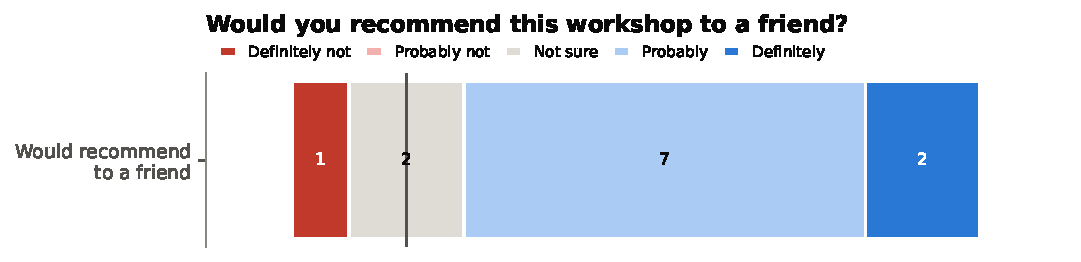
\includegraphics[width=0.92\linewidth]{fig/fig_recommend.pdf}
  \captionof{figure}{Willingness to recommend the workshop to a friend (counts of 12).}
\end{center}

% =============================================================================
\section*{1.\quad Who we heard from}

Twelve students completed the anonymous exit survey. The group was split across grades~9--11,
and most arrived with little or no formal economics background---so the gains below start
from a near-beginner baseline.

\begin{table}[htbp]
\centering
\small
\begin{tabular}{@{}llc@{}}
\toprule
\textbf{Characteristic} & \textbf{Most common response (mode)} & \textbf{Respondents} \\
\midrule
Grade (this fall)            & Grade 10                  & 6 of 12 \\
Prior econ / finance exposure & A little, informally     & 5 of 12 \\
Prior interest (1--5)         & Somewhat interested $=3$ & 4 of 12 \\
\bottomrule
\end{tabular}
\caption{Respondent profile ($n=12$): most common response to each question.}
\end{table}

% =============================================================================
\section*{2.\quad What worked best}

\subsection*{2.1\quad Teaching was rated highly}

Every teaching statement drew majority agreement. Students were most positive about the
\textbf{open, question-friendly classroom} and \textbf{clear explanations}---the two items
where 92\% agreed or strongly agreed.

\begin{figure}[htbp]
\centering
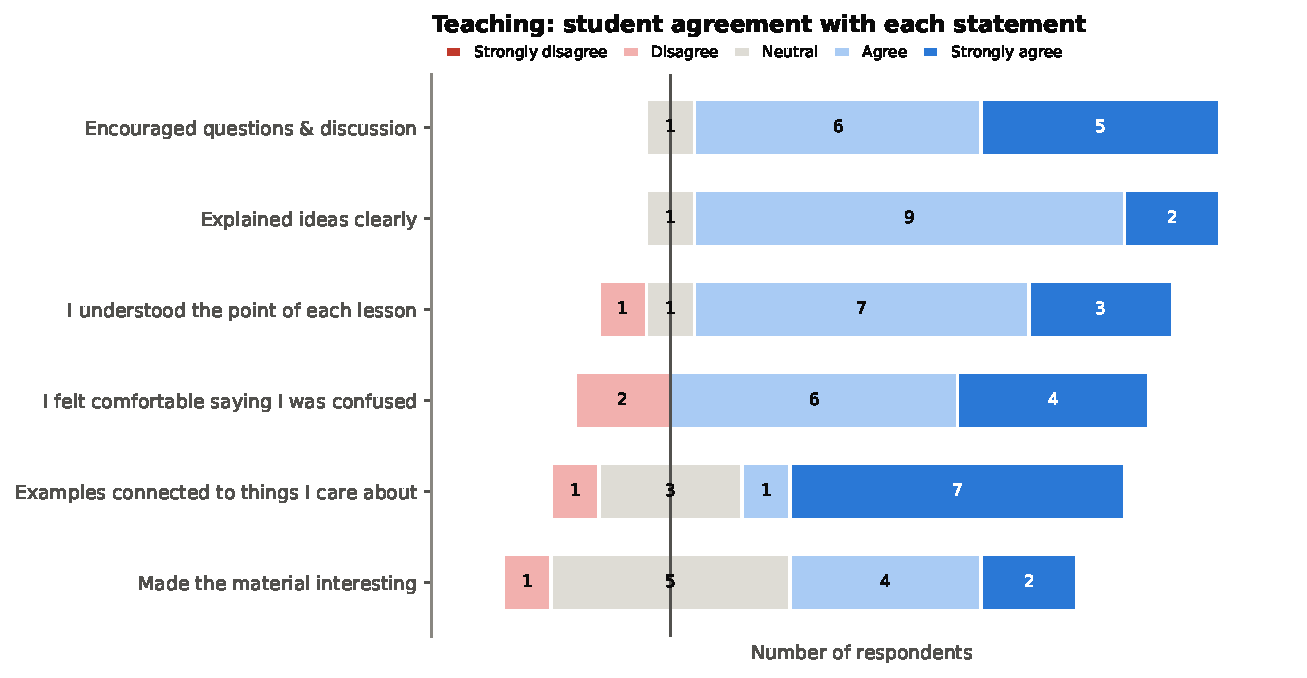
\includegraphics[width=\linewidth]{fig/fig_teaching.pdf}
\caption{Agreement with each teaching statement (counts of 12 respondents), best-rated at top.}
\end{figure}

\begin{table}[htbp]
\centering
\small
\begin{tabular}{@{}lcc@{}}
\toprule
\textbf{Teaching statement} & \textbf{Mean (1--5)} & \textbf{\% Agree (4--5)} \\
\midrule
Encouraged questions \& discussion            & 4.33 & 92\% \\
Examples connected to things I care about      & 4.17 & 67\% \\
Explained ideas clearly                        & 4.08 & 92\% \\
I understood the point of each lesson          & 4.00 & 83\% \\
I felt comfortable saying I was confused       & 4.00 & 83\% \\
Made the material interesting                   & 3.58 & 50\% \\
\midrule
\textbf{Overall}                                & \textbf{4.03} & \\
\bottomrule
\end{tabular}
\caption{Teaching ratings, highest mean first.}
\end{table}

\subsection*{2.2\quad Attitudes shifted toward relevance}

The workshop moved the needle most on \textbf{relevance}: three-quarters of students left
seeing economics as more connected to daily life and to how governments make policy.

\begin{figure}[htbp]
\centering
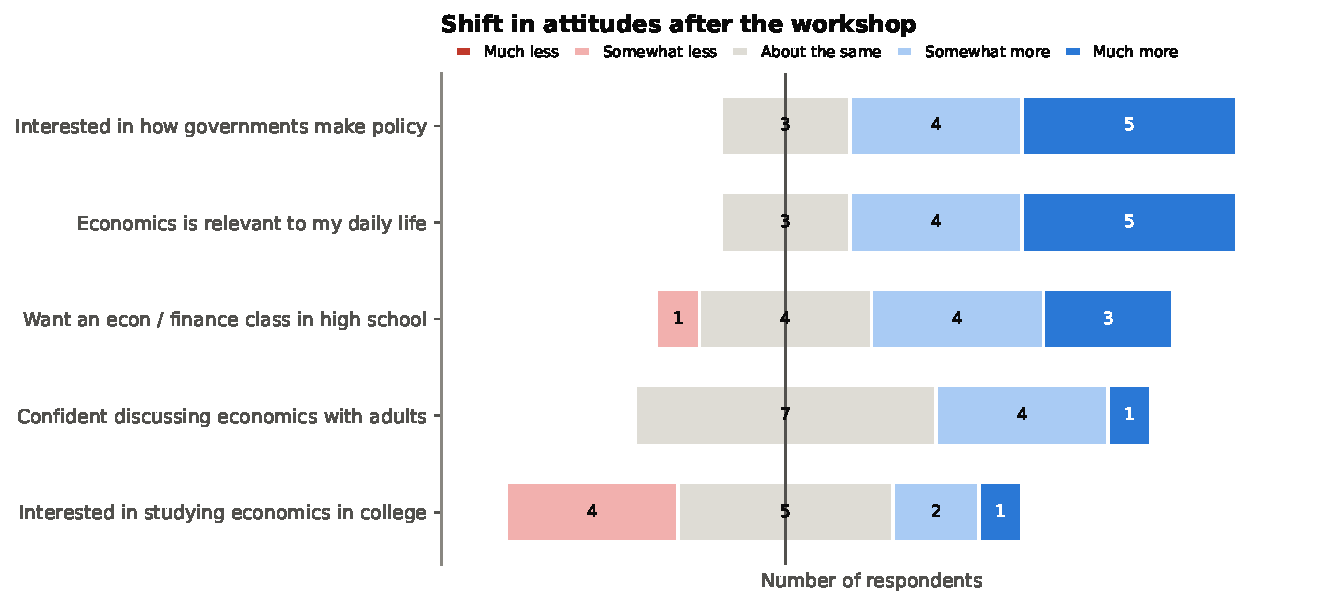
\includegraphics[width=\linewidth]{fig/fig_attitude.pdf}
\caption{Self-reported change in attitudes since before the workshop (counts of 12).}
\end{figure}

\begin{table}[htbp]
\centering
\small
\begin{tabular}{@{}lcc@{}}
\toprule
\textbf{Since the workshop, I feel\ldots} & \textbf{Mean (1--5)} & \textbf{\% ``More'' (4--5)} \\
\midrule
Economics is relevant to my daily life         & 4.17 & 75\% \\
Interested in how governments make policy      & 4.17 & 75\% \\
Want an econ / finance class in high school    & 3.75 & 58\% \\
Confident discussing economics with adults     & 3.50 & 42\% \\
Interested in studying economics in college    & 3.00 & 25\% \\
\bottomrule
\end{tabular}
\caption{Attitude shift (5 = much more than before).}
\end{table}

\newpage
\subsection*{2.3\quad Day 1 hooked them; Day 5 was most useful}

Day~1 (Economic Decision-Making) was the standout opener, marked ``interesting'' by
two-thirds of students. The financial-literacy content on Day~5---and the trade material on
Day~4---were most often marked ``useful outside school.'' Reassuringly, no single day was
widely flagged as hard.

\begin{figure}[!htp]
\centering
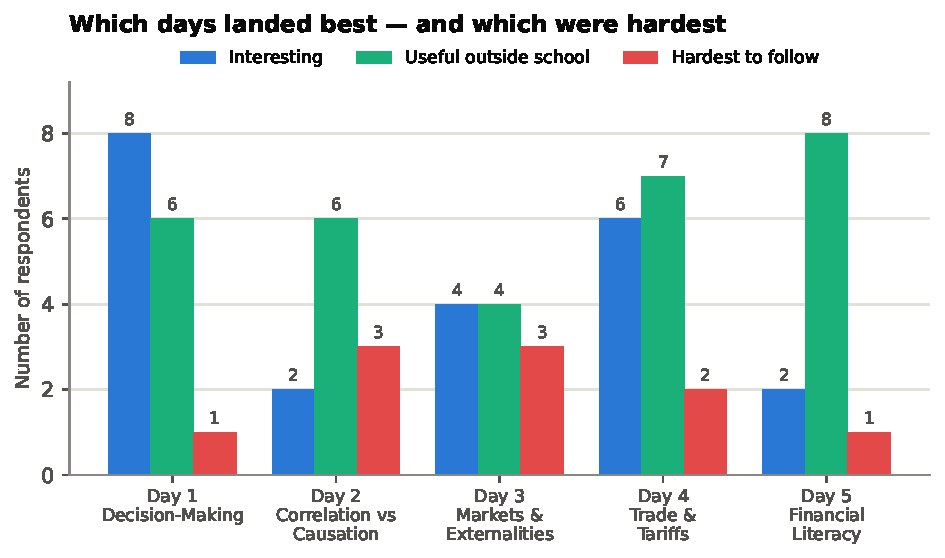
\includegraphics[width=\linewidth]{fig/fig_days.pdf}
\caption{Votes per day for interesting, useful, and hardest to follow. Students marked every day that applied in each column, not a single choice.}
\end{figure}

\subsection*{2.4\quad Learning by doing (and by news)}

When asked which ways of learning helped most, students favored \textbf{real-world news
examples}, \textbf{discussion}, and \textbf{games and simulations} over slides---a clear
signal about where to invest classroom time.

\begin{figure}[htbp]
\centering
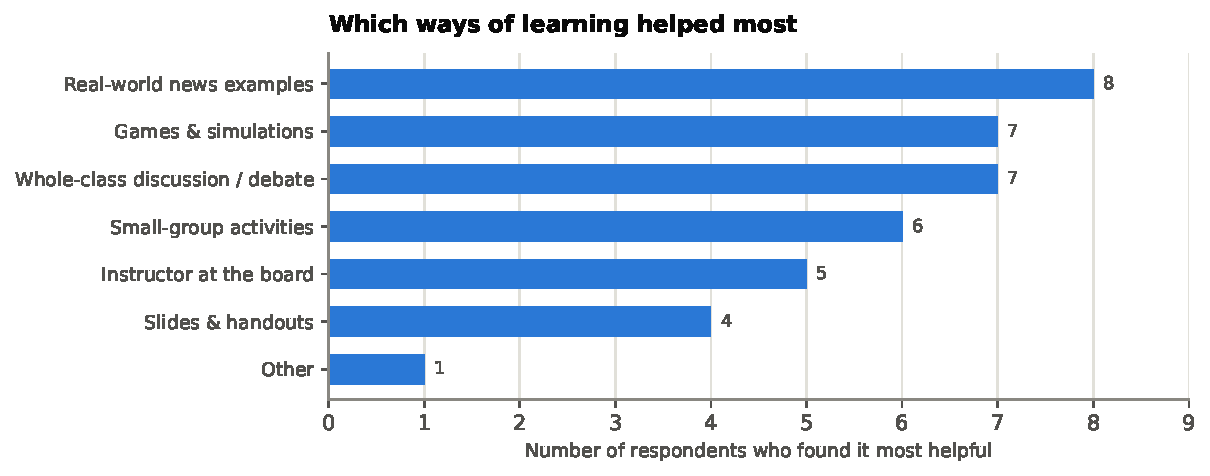
\includegraphics[width=\linewidth]{fig/fig_learning.pdf}
\caption{Ways of learning students found most helpful (each could choose up to two; several chose more).}
\end{figure}

\subsection*{2.5\quad Most would recommend it}

\noindent Three-quarters of students (9 of 12) would ``probably'' or ``definitely'' recommend
the workshop (see the headline chart on page~1). The single ``definitely not'' came from a
student who noted they had not chosen to enroll---an enrollment-fit issue rather than a comment
on the teaching.

% =============================================================================
\section*{3.\quad Where to improve}

\begin{enumerate}[label=\textbf{\arabic*.},itemsep=3pt,topsep=2pt]
  \item \textbf{Make it \emph{feel} as interesting as it is useful.} ``Made the material
        interesting'' was the only teaching item below 4.0 (mean 3.58; just 50\% agreed, with
        5 students neutral). The open feedback points the same way: students asked for more
        ``fun and interactive'' and ``hands-on'' lessons.
  \item \textbf{Break hard concepts into small gradual steps.} Day~2 (Correlation vs.\ Causation) and Day~3
        (Markets \& Externalities) were each flagged ``hardest to follow'' by 3 students---the
        most of any days. Extra worked examples and mid-lesson checks would help.
  \item \textbf{Build confidence and the college bridge.} Confidence discussing economics with
        adults barely moved (58\% ``about the same''), and interest in \emph{studying economics
        in college} was the weakest outcome (25\% up; 4 students dipped). The workshop built
        relevance far more than it built a sense of ``this could be my path.''
  \item \textbf{Give them concrete tools.} The most specific request was practical: how to
        actually invest. Adding a short, concrete ``how to start investing'' toolkit would meet
        real demand.
\end{enumerate}

% =============================================================================
\section*{4.\quad In students' own words}

\begin{quotebox}
``This was a really interesting lesson\ldots\ This class was important to me because I'm getting
into the financial world. I liked it, thank you so much.'' \hfill --- \textit{recommended: definitely}
\end{quotebox}

\begin{quotebox}
``The small-group activities helped motivate me to think with different perspectives. Sharing out
ideas was also helpful.'' \hfill --- \textit{recommended: definitely}
\end{quotebox}

\begin{quotebox}
``This class was much more interesting than I had originally anticipated---great job!'' \hfill --- \textit{recommended: probably}
\end{quotebox}

\noindent\textbf{Constructive:}
\begin{quotebox}
``I think more hands-on aspects would make this class more engaging, such as the candy example.''
\hfill --- \textit{recommended: probably}
\end{quotebox}

\begin{quotebox}
``It would be nice to make it more fun and interactive.'' \hfill --- \textit{recommended: not sure}
\end{quotebox}

% =============================================================================
\section*{5.\quad Recommendations}

\begin{enumerate}[label=\textbf{\arabic*.},itemsep=3pt,topsep=2pt]
  \item \textbf{Lead with what already works:} shift more time into games, simulations, and
        real-world news, and convert board-time into hands-on activities---these are exactly the
        modes students rated most helpful.
  \item \textbf{Add a concrete investing segment} (a short, practical ``how to start'' toolkit)
        to satisfy the clearest student request.
  \item \textbf{Break hard concepts into small gradual steps on Days~2--3}, with additional
        worked examples and quick comprehension checks to lower the difficulty spikes.
  \item \textbf{Grow confidence through student voice:} more student-led discussion and brief
        share-outs, so students practice talking economics aloud.
  \item \textbf{Bridge to ``what's next'':} a short segment on econ/finance pathways (courses,
        careers) to lift interest in studying the subject further.
\end{enumerate}

\vspace{1em}
\noindent\rule{\textwidth}{0.4pt}\\[0.3em]
{\footnotesize\textit{Method note.} Findings are based on 12 anonymous two-page exit surveys
collected on the final day. Each form was transcribed and independently spot-checked; percentages
are of 12 respondents and Likert items are coded 1--5. With a small sample, results are best read
as directional signals rather than precise estimates.}

\end{document}
